The device fabrication consists of four main processes. Included in these processes are various lithography steps, evaporation of different metals, wet etching and deposition of silicon nitride as an anti-reflective coating. First, one part the desired antenna structure is imprinted on a wafer through contact lithography and the first metal deposition step with chromium and gold is carried out. Then, mesa lithography and mesa etching is applied. Another lithography step for the rest of the antenna structure is executed, followed by the deposition of NiCr. In the end, an anti-reflective coating is deposited. 

\subsection{Antenna Structure Lithography and Deposition of Gold and Chromium}

\begin{figure}[h]
    \centering
    \begin{subfigure}[b]{0.225\textwidth}
        \centering
        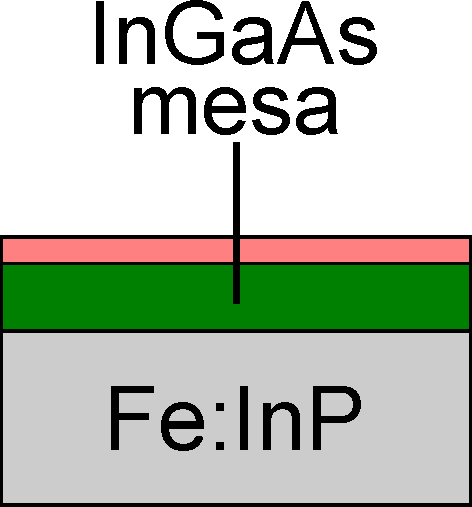
\includegraphics[width=\textwidth]{figures/Fabrication/fab1_1.pdf}
        \caption{}
        \label{fig:fab11}
    \end{subfigure}
    \hfill
    \begin{subfigure}[b]{0.225\textwidth}
        \centering
        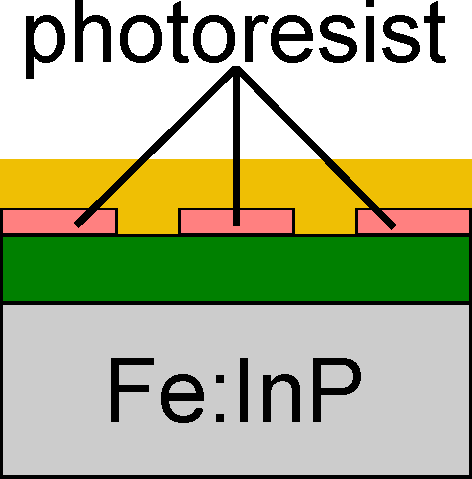
\includegraphics[width=\textwidth]{figures/Fabrication/fab1_2.pdf}
        \caption{}
        \label{fig:fab12}
    \end{subfigure}
    \hfill
    \begin{subfigure}[b]{0.225\textwidth}
        \centering
        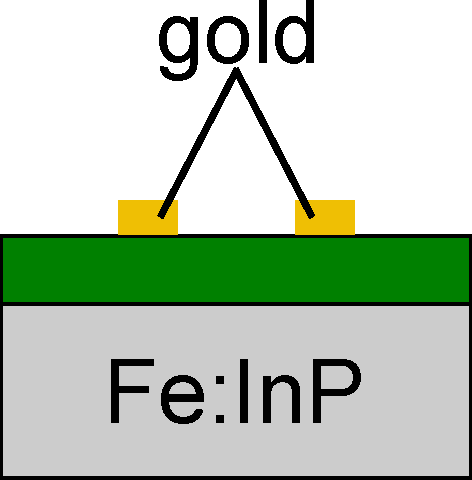
\includegraphics[width=\textwidth]{figures/Fabrication/fab1_3.pdf}
        \caption{}
        \label{fig:fab13}
    \end{subfigure}
    \caption{Schematic diagram depicting the principle steps of structure lithography and metal deposition. (a) The wafer is covered in AZ 5214E photoresist. (b) UV exposure leaves behind a patterned photoresistive structure. A metal layer is deposited through metal evaporation on top of the photoresistive layer. (c) Lift-off is performed to get rid of the excess metal. Left behind is only the metal in contact with the semiconducting material.}
\end{figure}

A lithography mask is fabricated containing the desired antenna structures. A \num{7} $\times$ \num{8} \si{\milli\meter} sample of an InGaAs photoconductor, grown on a \num{500} \si{\micro\meter} InP:Fe substrate wafer is cleaved out from the wafer. In the following steps, structures as small as \num{5} \si{\micro\meter} are desired, so good contact and alignment are critical.

% The desired antenna structures are imprinted onto the sample via contact lithography. Structures as small as approximately \num{1} \si{\micro\meter} are desired, so good contact is critical in this process. 

First, a fabrication step called zero-leveling is executed. The zero-leveling helps in achieving good contact when applying contact lithography. A thin layer of AZ 5214E image reversal photoresist is deposited onto the sample. By spin coating the sample at 8000 rpm, a uniform layer of photoresist is achieved. The image reversal effect of AZ 5214E is achieved by baking the sample at \num{110} \si{\celsius} (soft baking) for one minute and exposing it to ultraviolet (UV) light for \num{35} seconds. The sample is developed using AZ MIF 720, leaving a \num{6} $\times$ \num{7} \si{\milli\meter} area of photoresist.
A second lithographic step is performed to expose one part the antenna structures. The lithography mask is applied to the sample, which is then exposed to UV light for \num{3} seconds, followed by another soft baking step. A second UV exposure is carried out with five times the initial exposure duration. The sample is developed using AZ MIF 720, leaving behind the patterned antenna structures ready for gold deposition. 

The antenna structures are fabricated through metal deposition. In the first metal deposition step, gold structures are deposited on top of a chromium adhesion layer. Before depositing the metal for the PCAs, the samples are dipped into a 1:1 solution of H\textsubscript{2}O and HCl for \num{15} seconds to remove the oxide layer which forms at the surface. This step greatly improves the adhesion of the deposited metal. The antenna electrodes, contact pads and some part of the feeding strip are fabricated by depositing a \num{120} \si{\nano\meter} layer of gold (Au) on top of a \num{20} \si{\nano\meter} layer of Chrome (Cr) via electron beam evaporation. Cr is deposited at a rate of $\sim 0.3$ \si{\angstrom}/\si{\s}, Au is deposited at a rate of $\sim 0.8$ \si{\angstrom}/\si{\s}. The Cr-layer improves the contact with the semiconducting material. After completing the metal deposition, the sample is dipped in acetone. This way we get rid of the unwanted metal on our sample. 

An additional annealing step is performed after metal deposition to further improve the metal-semiconductor-contact. Such an annealing process reduces the interface impurities and creates good contact on the atomic scale between the metal and the semiconducting material \cite{tahamtanInvestigationEffectAnnealing2011}. Metal atoms diffuse into the InGaAs, making sure that we get an ohmic contact rather than a Schottky contact. Annealing is performed at a temperature of $\sim 422$ \si{\celsius} for \num{30} seconds at a pressure of \num{2} \si{\milli \bar}. 

\subsection{Mesa Lithography and Mesa Etching}

A layer of AZ 1518 HS photoresist is deposited onto the sample. Spin coating at 4000 rpm ensures a uniform photoresistive layer. Several lithography steps are performed before hard baking the sample covered in photoresist at \num{110} \si{\celsius} for \num{15} minutes. The hard baking makes the residual solvent present in the resist evaporate, stabilizes the printed structure and improves the bond between the resist and the material. 

The InGaAs photoconductive material is etched from the areas that were not protected by the photoresist layer using 
sulfuric acid (H\textsubscript{2}SO\textsubscript{4}), hydrogen peroxide (H\textsubscript{2}O\textsubscript{2}) and water (H\textsubscript{2}0) mixed in appropriate proportion. We use a ratio of \num{1} \si{\milli \liter} : \num{8} \si{\milli \liter} : \num{50} \si{\milli \liter} respectively. The semi-insulating InP:Fe substrate is left exposed in those areas. 

By mesa etching, the active InGaAs layer is removed from the entire sample except between the electrodes and under the antenna and pads. This process ensures a high resistance with a minimal dark current. A minimal dark current drastically improves the signal-to-noise ratio of the THz signal. 

\begin{figure}[h]
    \centering
    \begin{subfigure}[b]{0.225\textwidth}
        \centering
        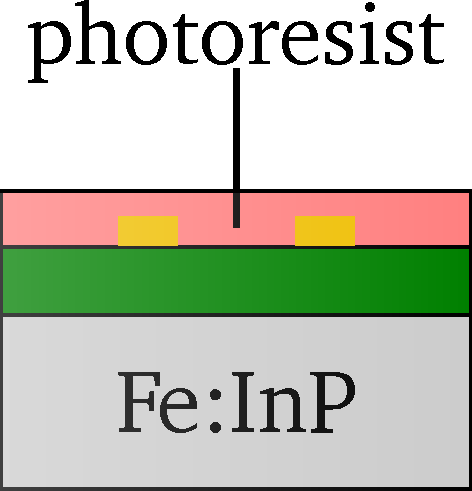
\includegraphics[width=\textwidth]{figures/Fabrication/fab2_1.pdf}
        \caption{}
        \label{fig:fab21}
    \end{subfigure}
    \hfill
    \begin{subfigure}[b]{0.225\textwidth}
        \centering
        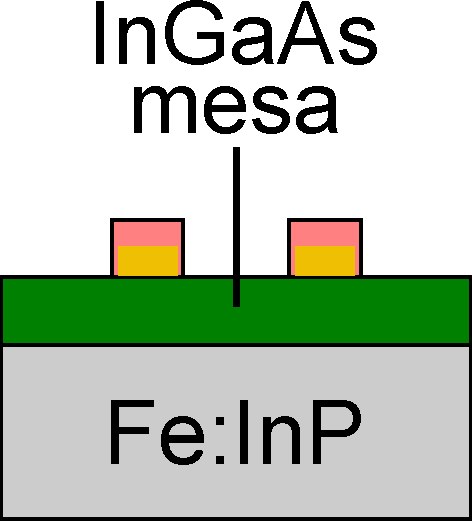
\includegraphics[width=\textwidth]{figures/Fabrication/fab2_2.pdf}
        \caption{}
        \label{fig:fab22}
    \end{subfigure}
    \hfill
    \begin{subfigure}[b]{0.225\textwidth}
        \centering
        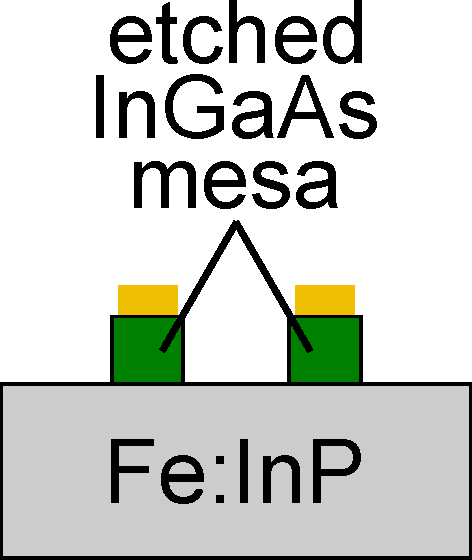
\includegraphics[width=\textwidth]{figures/Fabrication/fab2_3.pdf}
        \caption{}
        \label{fig:fab23}
    \end{subfigure}
    \caption{Schematic diagram depicting the principle steps of structure lithography and metal deposition. (a) The wafer is covered in AZ 5214E photoresist. (b) UV exposure leaves behind a patterned photoresistive structure. A metal layer is deposited through metal evaporation on top of the photoresistive layer. (c) Lift-off is performed to get rid of the excess metal. Left behind is only the metal in contact with the semiconducting material.}
\end{figure}


\subsection{Antenna Structure Lithography and Deposition of NiCr}
This step is similar to the metal deposition of Au and Cr. The desired structures are imprinted onto the sample through photo-lithography. The imprinted structures are the missing parts of the feeding strips connecting antenna pads and electrodes. Good contact between the NiCr-strip and the AuCr-strip is vital. Otherwise, THz performance will decrease drastically. We spin coat the sample with nLof 2035 at \num{4000} rpm. The sample is soft baked, exposed to UV light and developed using AZ MIF 720. Left behind are the missing parts of the antenna feeding strips, ready for NiCr deposition.

A \num{80}/\num{20} NiCr alloy is deposited onto the sample using flash evaporation. Flash evaporation of \num{80}/\num{20} NiCr involves the rapid heating of the alloy in an evacuated environment (around $10^{-9}$ \si{\bar}). NiCr has a high melting point around \num{1450} \si{\celsius}. The alloy has to be heated rapidly to avoid clumps and bulk melting, assuring a thin, uniform NiCr layer on top of the sample. Constantly adjusting the feed rate of the alloy also helps in avoiding bulking. Ultimately, the deposition rate should be kept around \num{0.3} \si{\angstrom}/\si{\s}. As Nickel and chromium have slightly different melting temperatures it is also vital to make sure that the two metals are evaporated at equal rates. Upon reaching its evaporation temperature, the NiCr vaporizes, travels through the vacuum and condenses onto the sample. Figure \ref{PCA_NICR} depicts a schematic of the antenna structure after flash evaporation of NiCr. 

\begin{figure}[ht]
    \centering
    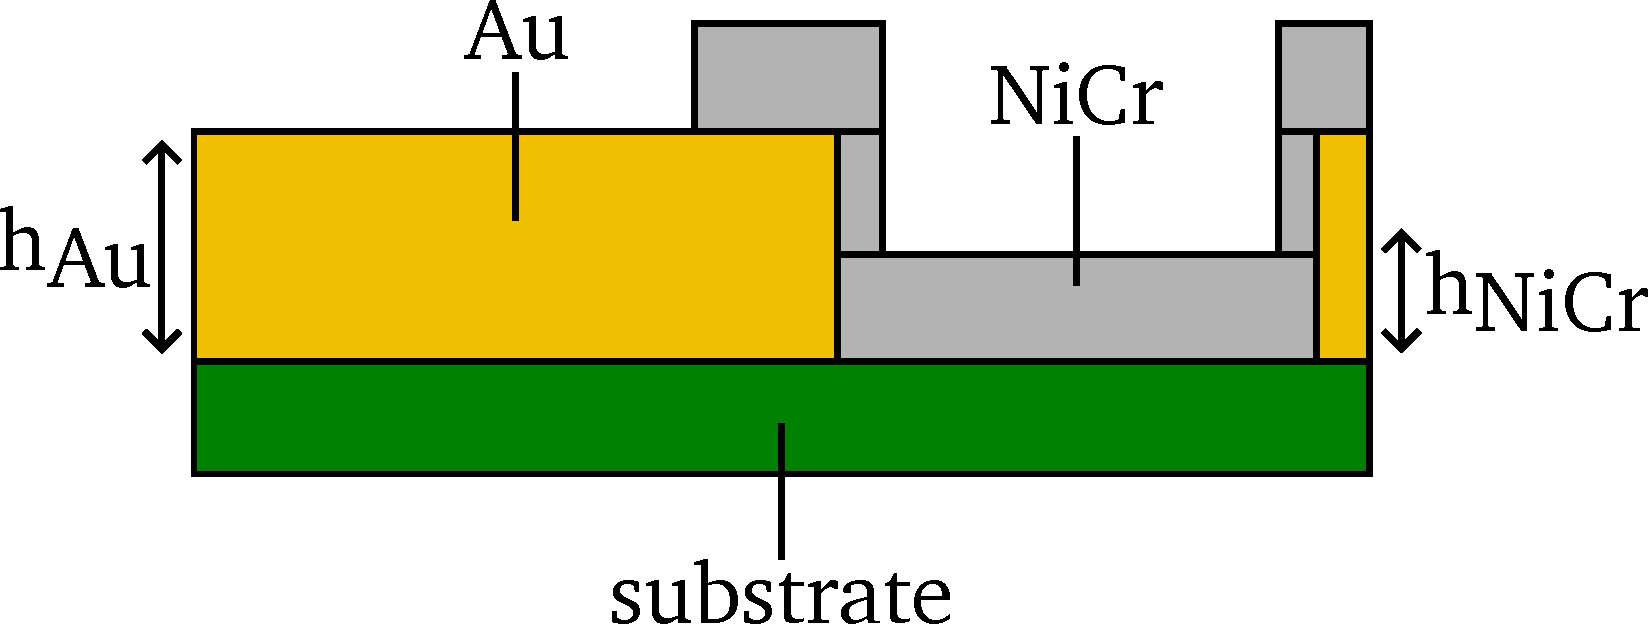
\includegraphics[width=0.8\textwidth]{figures/Fabrication/PCA_after_NiCr.pdf}
    \caption{Schematic side view of a section of a PCA after NiCr deposition. Au and NiCr are deposited at different heights: $h_{Au} \approx 140$ \si{\nano \meter}, $h_{NiCr} \approx 90$ \si{\nano \meter}. Not to scale.}
    \label{PCA_NICR}
\end{figure}

\subsection{Anti-Reflection Coating Deposition}
An anti-reflection coating (ARC) is deposited above the active region. The ARC layer helps improving the transmission of the THz by minimizing reflection \cite{chenAntireflectionImplementationsTerahertz2014} and protects the device from external damage. The ARC is fabricated by growing a silicon nitride (Si\textsubscript{3}N\textsubscript{4}) layer on top of the sample via plasma-enhanced chemical vapor deposition. 

After depositing the ARC, another layer of AZ 1518 HS photoresist is deposited onto the sample to form the required shapes of the ARC over the mesa. The photoresist only covers the antennas electrode structure. 

The Si\textsubscript{3}N\textsubscript{4} is etched out from the unprotected areas, exposing the contacting metal pads attached to the antenna. The etching is done in a plasma etching machine using carbon tetra-fluoride (CF\textsubscript{4}) as the etching agent. After etching of Si\textsubscript{3}N\textsubscript{4} the photoresist is removed by dipping the sample into acetone.


\textbf{TODO: ABBILDUNG maybe}